

\section{实验目的}
文件传输是计算机网络的基本功能,文件传输协议(FTP)是一个基本的应用层
协议.本实验要求在Linux 系统上使用Socket 编程技术实现简化的FTP 服务器和客
户端的程序,使客户端可以连接至服务器,并且可以进行一些FTP 的基本操作,如
列出目录、下载文件等.

\section{实验原理}

FTP 是File Transfer Protocol,即文件传输协议的缩写.该协议用于在两台计算机
之间传送文件.基本模型如下:
\begin{figure}[H]
  \centering
  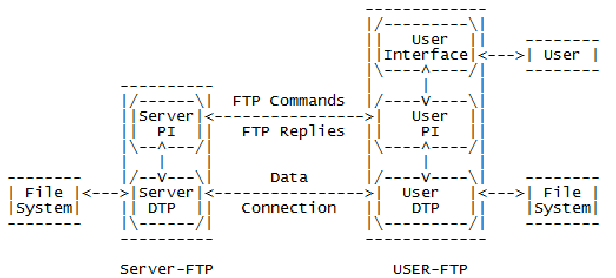
\includegraphics[width=\textwidth]{res/ftp1.png}
\end{figure}

FTP 会话包含两个TCP 连接通道,一个是控制通道,一个是数据通道.如下图
所示:
\begin{figure}[H]
  \centering
  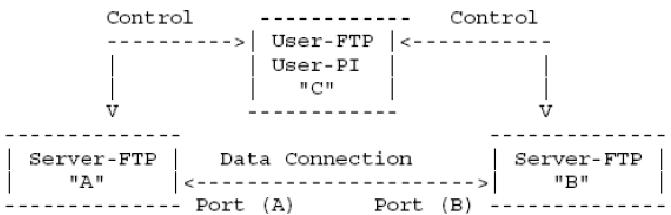
\includegraphics[width=\textwidth]{res/ftp2.png}
\end{figure}

控制通道是和FTP 服务器进行沟通的通道,连接FTP 服务器,发送FTP 指令;
数据通道则是和FTP 服务器进行文件传输或者获取文件列表的通道.
FTP 协议中控制连接的各种指令均由客户端主动发起,而数据连接有两种工作
方式:主动方式(PORT 方式)和被动方式(PASV 方式).主动方式下,FTP 客户
端首先和FTP 服务器的控制通道对应端口(一般为21)建立连接,通过控制通道发
送命令客户端需要接收数据的时候在这个通道上发送PORT 命令.PORT命令包含了
客户端用什么端口(一个大于1024 的端口)接收数据.在传输数据的时候,FTP 服
务器必须和客户端建立一个新的连接,服务器通过自己的TCP20端口发送数据.被
动方式下,建立控制通道的过程和主动方式类似,当客户端通过这个通道发送PASV
命令的时候, FTP server 打开一个位于1024$ \sim$5000 之间的随机端口并且通知客户端,
然后客户端与服务器之间将通过这个端口进行数据的传送.如下图所示:


\begin{figure}[H]
  \centering
  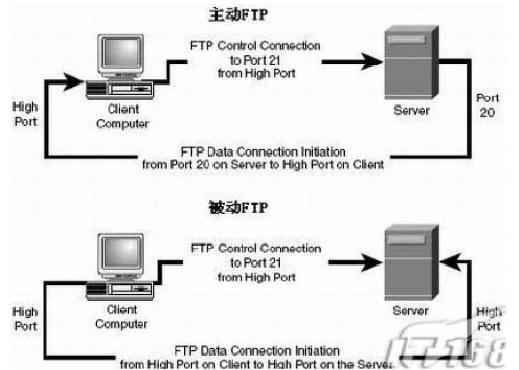
\includegraphics[width=0.8\textwidth]{res/ftp3.png}
\end{figure}


FTP 的工作流程如下:
\begin{enumerate}[(1)]
    \item FTP 服务器运行守护进程,等待FTP 请求.
    \item 它收到客户端的FTP 请求以后,建立控制连接,等待客户端命令.
    \item 如果服务器收到正确的传输文件命令,则新开一个数据连接,使用另外的端口进行传输.数据传输完以后,关闭数据连接.
    \item 如果服务器收到其他命令,则根据不同的命令做出响应.
    \item 如果收到quit 命令,结束控制连接,结束会话.
\end{enumerate}
